\documentclass[a4paper,11pt]{scrartcl}
\usepackage[margin=1in]{geometry}
\usepackage{listings}
\usepackage{longtable}
\usepackage{tabularx}
\usepackage{graphicx}
\usepackage[x11names,dvipsnames,table]{xcolor}
\usepackage{amsmath}
\usepackage{amssymb}
\usepackage{calc}
\setlength{\parindent}{0pt}

\newcommand{\asmenv}[1] {
    \rowcolors{1}{lightgray}{white}
    \begin{longtable}{ll}
    #1
    \end{longtable}
}

\newcommand{\asmr}[2] {
    \texttt{#1} & \text{#2} \\
}

\newcounter{stkctr}
\newcommand{\stackenv}[1]{
    \setcounter{stkctr}{0}
    \rowcolors{1}{lightgray}{white}
    \begin{tabular}{|c|l|l|l|}
        \hline
    Frame & Adress & Contents & Meaning \\
    \hline
    #1
    \end{tabular}
}

\newcommand{\stackframe}[2]{
    \texttt{#1} & & & \\
    #2
    \hline
}

\newcommand{\stackrow}[2]{
    & \texttt{b - \thestkctr} & \texttt{#1} & \texttt{#2} \addtocounter{stkctr}{4} \\
}

\newcommand{\Proof}[2]{
    \rowcolors{1}{white}{white}
    \begin{minipage}[t]{\linewidth}
    \underline{Claim:}
    #1
    \end{minipage}

    \leavevmode
    \\

    \begin{minipage}[t]{\linewidth}
    \underline{Proof:}
    #2 $\blacksquare$
    \end{minipage}

    \leavevmode
    \\
}

\newcommand{\Induction}[2]{
    \rowcolors{1}{white}{white}

    \textit{BC:}
    \newlength{\bcaselen}
    \settowidth{\bcaselen}{\textit{BC:....}}
    \begin{minipage}[t]{\linewidth-\bcaselen}
    #1
    \end{minipage}

    \leavevmode
    \\

    \textit{IS:}
    \newlength{\indsteplen}
    \settowidth{\indsteplen}{\textit{IS:....}}
    \begin{minipage}[t]{\linewidth-\indsteplen}
    #2
    \end{minipage}

    \leavevmode
    \\
}

\begin{document}

The rules mentioned (on lines 1, 4, 6, 9, 17, 22, 36–40, 42–44 and 49), without semantic actions (which make them all distinct), are:

\enumerate{
\item $reg  \rightarrow \langle Const\text{ } k \rangle$ (when fits move k)
\item $reg  \rightarrow \langle Local\text{ } n \rangle$ (when fits add n)
\item $reg  \rightarrow \langle Global\text{ } x \rangle$
\item $reg  \rightarrow \langle Loadw, addr \rangle$
\item $reg  \rightarrow \langle Binop\text{ } PlusA, reg1 , rand \rangle$
\item $reg  \rightarrow \langle Binop\text{ } Lsl, reg1, rand \rangle$
\item $rand \rightarrow \langle Const\text{ } k \rangle$ (when fits immed k)
\item $rand \rightarrow \langle Binop\text{ } Lsl, reg, \langle Const\text{ } n \rangle \rangle$ (when $n < 32$)
\item $rand \rightarrow \langle Binop\text{ } Lsl, reg1, reg2 \rangle$
\item $rand \rightarrow reg$
\item $addr \rightarrow \langle Local\text{ } n \rangle$ (when fits offset n)
\item $addr \rightarrow \langle Binop\text{ } PlusA, reg1, reg2 \rangle$
\item $addr \rightarrow \langle Binop\text{ } PlusA, reg1, \langle Binop\text{ } Lsl, reg2, \langle Const\text{ } n \rangle \rangle \rangle$ (when $n < 32$)
\item $addr \rightarrow reg$
\item $stmt \rightarrow \langle Storew, reg, addr \rangle$
}

\leavevmode
\\

Now to systematically calculate in how many ways we can tile the tree with these rules, we use dynamic programming:
\begin{itemize}
\item For each node $i$, and each symbol $S \in \{ stmt, addr, rand, reg \}$ we calculate $d_i^S$, the number of ways in which we can tile the subtree with it's root at $i$, and such that the tree can be generated from the symbol $S$, from bottom to top.
\item To find $d_i^S$, assuming that $d_j^\_$ has been found for all nodes $j \ne i$ in the subtree of $i$, use the following formula: \\
$d_i^S = \sum\limits_{\text{Pattern } p \text{ for } S \text { matches subtree at } i} (\prod\limits_{X \text{non-terminal in p}} d_{\text{node of } X}^X)$
\end{itemize}
\leavevmode
\par

The answer is in $d_{root}^{stmt}$. \\
\newpage
Numbering the nodes as in the diagram, the table holds synthesizes the information found by the dynamic programming algorithm:

\begin{minipage}[c]{.5\textwidth}
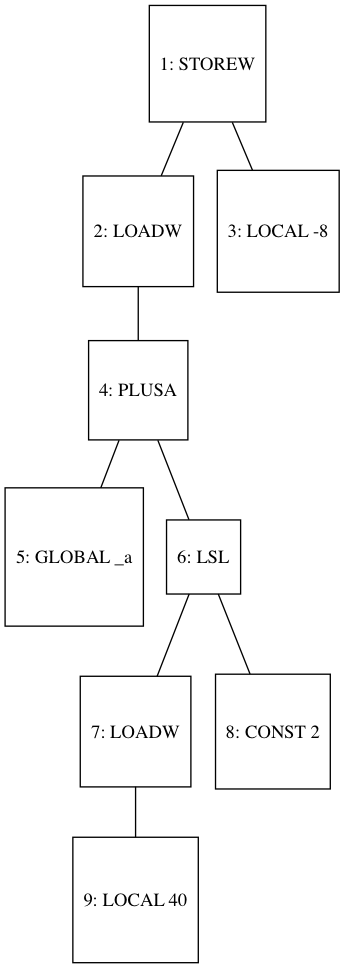
\includegraphics[width=.7\textwidth]{ex1.png}
\end{minipage}
\begin{minipage}[c]{.5\textwidth}
\begin{tabular}{|c|c|c|c|}

\hline
Node $i$ & Symbol $S$ & Rules & $d_i^S$ \\
\hline
1 & reg & & 0 \\
\hline
1 & rand & 10 & 0 \\
\hline
1 & addr & 14 & 0 \\
\hline
1 & stmt & 15 & \underline{28} \\
\hline

2 & reg & 4 & 14\\
\hline
2 & rand & 10 & 14\\
\hline
2 & addr & 14 & 14\\
\hline
2 & stmt & & 0 \\
\hline

3 & reg & 2 & 1\\
\hline
3 & rand & 10 & 1\\
\hline
3 & addr & 11, 14 & 2\\
\hline
3 & stmt & & 0 \\
\hline

4 & reg & 5 & 8\\
\hline
4 & rand & 10 & 8\\
\hline
4 & addr & 12, 13, 14& 14 \\
\hline
4 & stmt & & 0 \\

\hline
5 & reg & 3 & 1\\
\hline
5 & rand & 10 & 1\\
\hline
5 & addr & 14 & 1\\
\hline
5 & stmt & & 0 \\
\hline

6 & reg & 6 & 4\\
\hline
6 & rand & 8, 9, 10& 8\\
\hline
6 & addr & 14 & 4 \\
\hline
6 & stmt & & 0 \\
\hline

7 & reg & 4 & 2 \\
\hline
7 & rand & 10 & 2 \\
\hline
7 & addr & 14 & 2 \\
\hline
7 & stmt & & 0 \\
\hline

8 & reg & 1 & 1 \\
\hline
8 & rand & 7, 10 & 2 \\
\hline
8 & addr & 14 & 1\\
\hline
8 & stmt & & 0 \\
\hline

9 & reg & 2 & 1 \\
\hline
9 & rand & 10 & 1 \\
\hline
9 & addr & 11, 14& 2\\
\hline
9 & stmt & & 0 \\
\hline
\end{tabular}
\end{minipage}
So the answer is that there are 28 different tilings. \\

By inspecting all 28 trees, I've found that the shortest code is precisely the one in the notes:

\begin{lstlisting}{language=arm}
ldr r0, =_a
ldr r1, [fp, #40]
lsl r1, r1, #2
ldr r0, [r0, r1]
str r0, [fp, #-8]
\end{lstlisting}

And that the worst code is the one that uses the least specific rule at each possible choice (i.e. splits each node into its own tile), and that stores all temporary values in registers:

\begin{lstlisting}{language=arm}
ldr r0, [fp, #40]
ldr r1, [r0]
mov r2, #2
lsl r3, r1, r2
ldr r4, =_a
add r4, r4, r3
ldr r5, [r4]
ldr r6, [fp, #-8]
str r6, r0
\end{lstlisting}

This is almost the "bad" code from the notes, just that instead of directly computing \texttt{lsl r3, r1, \#2}, we first move \texttt{\#2} into a register and then compute this.

Assume pointers are 4 bytes and aligned to 4 bytes, and integers are 4 bytes and aligned to 4 bytes. \\
The record layout will be thus:
\begin{itemize}
\item 4 bytes for \texttt{data}
\item 4 bytes for \texttt{next}
\end{itemize}
and the record will be 4 byte aligned. \\

Suppose that the stack layout is thus:

\begin{itemize}
\item at fp - 8, the second local variable byte (supposijng it is 4 bytes long)
\item at fp - 4, the first local variable (supposing it is 4 bytes long)
\item at fp, the dynamic link
\item at fp + 4, the return address
\item at fp + 8, the beginning of the procedure currenty being run
\item at fp + 12, the static link
\item at fp + 16, the first argument
\item at fp + 20, the second argument
\item ...
\end{itemize}

\section{Problem 3}
I assume I don't have a \texttt{SWAP} instruction.

\begin{lstlisting}[language=Ml]

(* This function associates each instrution with the effect
 * it has on stack depth *)
let stack_depth_delta instruction = match instruction with
    BINOP w -> -1
    | MONOP w -> 0
    ...

(* This function computes the largest element in a list *)
let rec max_element ls = match ls with
    [x] -> x
    x :: xs -> max x (max_element xs)

(* This function finds the maximal stack depth for a certain
 * instruction sequence *)
let max_stack_depth ls =
    max_element
        (0 :: List.foldl (fun acc x -> acc + stack_depth_delta x) 0ls)

(* This will generate optimal code for expr, assuming that
 * the temporary variables v, v+1, ... are available,
 * using at most N stack positions. *)
let rec gen expr N v = match expr with
      Constant x ->
        CONST x
    | Variable x ->
        SEQ [LINE x.x_line; LDGW x.x_lab]
    | Monop (w, e1) ->
        SEQ [gen e1 N v; MONOP w]
    | Binop (w, e1, e2) ->
        let ins1 = gen e1 N (v+1)
        and ins2 = gen e2 N (v+1) in
        if max_stack_depth ins2 < N then
            SEQ [ins1; ins2; BINOP w]
        else
            SEQ [ins1; GET v ; ins2; PUT v ; BINOP w]

\end{lstlisting}

The following is a Keiko instruction sequence that implements the given statements:

\asmenv{
    \asmr{Instruction}{Stack after instruction}
    \asmr{LOCAL -8}{\&s}
    \asmr{LOADW}{s}
    \asmr{LOCAL -4}{s; \&q}
    \asmr{LOADW}{s; q}
    \asmr{LOADW}{s; q$\uparrow$.data}
    \asmr{PLUS}{s + q$\uparrow$.data}
    \asmr{LOCAL -8}{s + q$\uparrow$.data; \&s}
    \asmr{STOREW}{}
    \asmr{LOCAL -4}{\&q}
    \asmr{LOADW}{q}
    \asmr{CONST 4}{q; 4}
    \asmr{OFFSET}{q + 4}
    \asmr{LOADW}{q$\uparrow$.next}
    \asmr{LOCAL -4}{q$\uparrow$.next; \&q}
    \asmr{STOREW}{}
}

The associated trees are found in diagram 2.

\section{Problem 5}
\subsection{a}
A suitable representation is the type:
\begin{lstlisting}
type expr = Const of int
    | Var of string
    | Plus of expr * expr
    | Times of expr * expr
\end{lstlisting}
Assuming we have type:
\begin{lstlisting}
type code = CONST of int | LOAD of string | ADDMUL | SEQ of code list
\end{lstlisting}
which represents code in the vector machine, then a translation function would be:

\begin{lstlisting}[language=Ml]
let rec translate = function
    Const x -> CONST x
    | Var x -> LOAD X
    | Times x y ->
        SEQ [CONST 0; translate x; translate y; ADDMUL]
    | Plus x (Times y z) ->
        SEQ [translate x; translate y; translate z; ADDMUL]
    | Plus (Times x y) z ->
        SEQ [translate z; translate x; translate y; ADDMUL]
    | Plus x y -> SEQ [trasnlate x; translate y; CONST 1; ADDMUL]

\end{lstlisting}

\subsection{b}
\ASMEnv{
\ASMRow{Instruction}{Stack after instruction}
\ASMRow{CONST 0}{0}
\ASMRow{CONST 4}{0, 4}
\ASMRow{LOAD a}{0, 4, a}
\ASMRow{ADDMUL}{4 * a}
\ASMRow{CONST 0}{4 * a, 0}
\ASMRow{SWAP}{0, 4 * a}
\ASMRow{LOAD c}{0, 4 * a, c}
\ASMRow{ADDMUL}{4 * a * c}
\ASMRow{LOAD b}{4 * a * c, b}
\ASMRow{LOAD b}{4 * a * c, b, b}
\ASMRow{ADDMUL}{4 * a * c + b * b}
}

\subsection{c}
Suppose $e$ is some expression that requires a stack depth of $3$. Suppose $t$ is a sequence of instructions that calculates that $e$. Now, notice that if we calculate $e * e$ in a machine that allows arbitrary permutations of a bounded number of elements on the top of the stack, we can use a stack of depth at most $4$:

\ASMEnv{
\ASMRow{Instruction}{Stack after instruction}
\ASMRow{t}{e}
\ASMRow{t}{e, e}
\ASMRow{CONST 0}{e, e, 0}
\ASMRow{SWAP top with 3rd from top}{0, e, e}
\ASMRow{ADDMUL}{e * e}
}

(the stack depth of $4$ is reached when calculating $e$ for the second time).\\
(For simplicity I assumed that we can't "cheat" and just copy the value of e from the top of the stack again -- since any expression can be made into a structurally identical expression that evaluates to something different by changing some choice of variable or constant, this is justified).\\

Now, note that in a machine that can only swap the top $2$ values in the stack, the $0$ we require on the bottom of the stack in the final \texttt{ADDMUL} operation cannot be put there after the calculation of the second $e$. This means that we must first reach a stack state of \texttt{0, e} (by first calculating $e$, then pushing a $0$, then \texttt{SWAP}-ing), and then calculate $e$ again. Since calculating $e$ takes at least a stack of depth $3$, this procedure requires a stack of depth $4$.

\subsection{d}

Part (c) suggests that a sufficient instruction should be a \texttt{SWAP3} instruction, that swaps the top element of the stack with the 3rd element off the top (I think the reason why this is important has to do with the fact that these two swaps together can arbitrarily permute the top $3$ elements on the stack, and \texttt{ADDMUL} uses the top $3$ elements on the stack only).
The algorithm I suggest for generating the optimum has several cases:
\begin{itemize}
\item If we deal with constants or variablas, simply CONST or LOAD them onto the stack.
\item If we deal with an expression of the form $x * y$, then calculate $x$ and $y$ in the decreasing order of needed stack height, then push a $0$ onto the stack. Then, \texttt{SWAP3} the $0$ so that it is the $3^{rd}$ from the top, then \texttt{ADDMUL}
\item If we deal with an expression of the form $a*b + c*d$, w.l.o.g. suppose that evaluating $a*b$ takes more stack space then $c*d$. Then, first evaluate $a*b$ as before, then evaluate $c$, then $d$, then \texttt{ADDMUL}
\item If we deal with an expression of the form $x + c * d$ (or symmetrically $c * d + x$), evaluate $x$, then $c$, then $d$, then \texttt{ADDMUL}
\end{itemize}


\end{document}
